% CS 5306 / INFO 5306 Project 2 report.
% Build: nix run .#report   (or pdflatex/bibtex/pdflatex/pdflatex)
% Every number in this file comes from out/results.json.

\documentclass[sigconf,nonacm]{acmart}

\usepackage{booktabs}
\usepackage{graphicx}

\settopmatter{printacmref=false}
\renewcommand\footnotetextcopyrightpermission[1]{}
\pagestyle{plain}

\begin{document}

\title{Searching Before the Numbers Arrive: Nowcasting State Unemployment Claims from
Google and Reddit}
\subtitle{CS 5306 / INFO 5306, Project 2}

\author{Kevin Lei}
\affiliation{\institution{Cornell University}\country{}}
\email{kl2344@cornell.edu}

\author{Kyungmin Nam}
\affiliation{\institution{Cornell University}\country{}}
\email{kn467@cornell.edu}

\author{Brittany Sun}
\affiliation{\institution{Cornell University}\country{}}
\email{bs835@cornell.edu}

\begin{abstract}
The official count of new unemployment insurance claims for a week is published five days
after the week ends. Google searches and Reddit posts from the same week exist by Sunday. We
ask whether they improve a nowcast of weekly initial claims in California, Washington, New
York, and Texas beyond what past claims and the calendar already predict. We fit each model
only on earlier weeks and score it on 156 later weeks per state, October 2023 to September
2026. Adding Google Trends reduces squared nowcast error by $11.9\%$ across the four states,
by $23.2\%$ in California and $22.1\%$ in Texas, and not at all in Washington. The gain is
concentrated in a few weeks: holiday weeks, and above all the week Hurricane Beryl struck
Texas, when the search-augmented model halved the baseline's error. Excluding holiday weeks,
the gain is $7.9\%$. Posts in r/Unemployment tagged with a state add $1.4\%$. Our second
hypothesis, that tech-career discussion on Reddit helps more in California and Washington,
is not supported: it helps in no state.
\end{abstract}

\maketitle

\section{Introduction}

Every Thursday the U.S.\ Department of Labor reports how many people filed a new claim for
unemployment insurance in the week that ended the previous Saturday. Initial claims are
among the fastest official labor-market indicators, but they still arrive with a lag, and
in a shock the lag is when the information matters most. Meanwhile, people who lose their
jobs search for how to file, and some of them post about it.

Choi and Varian~\cite{choi2012predicting} showed that Google searches improve nowcasts of
national initial claims, and later work found the same for unemployment
rates~\cite{askitas2009google,damuri2017predictive} and for the 2020 claims
surge~\cite{goldsmith2020predicting}. Antenucci et al.~\cite{antenucci2014using} built a
claims index from tweets about job loss. The best-known failure is Google Flu Trends, which
tracked influenza well until it did not~\cite{ginsberg2009detecting,lazer2014parable}.
Lazer et al.\ found that part of its accuracy was seasonality that any calendar model would
have captured. We take that critique as a design constraint: an online signal earns credit
only for what it adds to a model that already knows the season, and only on weeks the model
was not fit on.

Our contribution is to repeat this test at the state level, for a recent period without a
pandemic-sized shock, and to add Reddit. We find that searches still help, but unevenly
across states and weeks, and that Reddit adds little.

\section{Data and Resources}
\label{sec:data}

\textbf{Initial claims.} Weekly initial claims, not seasonally adjusted, for the four states
from FRED~\cite{fredclaims}. A week runs Sunday to Saturday. Average weekly claims over our
window were $43{,}710$ in California, $16{,}360$ in New York, $15{,}843$ in Texas, and
$5{,}609$ in Washington. We use claims back to 2015 to construct the year-ago seasonal terms.

To nowcast honestly we need to know what a forecaster could have known on each Sunday. We
downloaded $1{,}044$ past versions of the series from ALFRED, FRED's archive of past
releases: each state's series as it appeared on every Sunday of the study period. Of $61{,}466$ weekly values compared with today's data, $4$ have
since been revised, all in Washington. The values are therefore final when first published.
On $10.6\%$ of Sundays, however, FRED had not yet posted the previous week's value. The
Department of Labor publishes it the preceding Thursday, so our main analysis assumes it is
known, and Section~\ref{sec:robust} reruns the comparison without it.

\textbf{Google Trends.} Weekly search interest~\cite{googletrends} for three terms in each
state: ``file for
unemployment'' and ``unemployment benefits'' (the terms from our proposal) and the broader
``unemployment''. Trends reports a 0--100 index scaled to the peak of the requested window,
not search counts. Weekly resolution is available only for windows under five years, so we
requested October 3, 2021 to September 26, 2026, which also sets our study period. In
Washington, ``file for unemployment'' is reported as zero in $33.2\%$ of weeks, because
Trends suppresses low volumes.

\begin{figure*}[t]
  \centering
  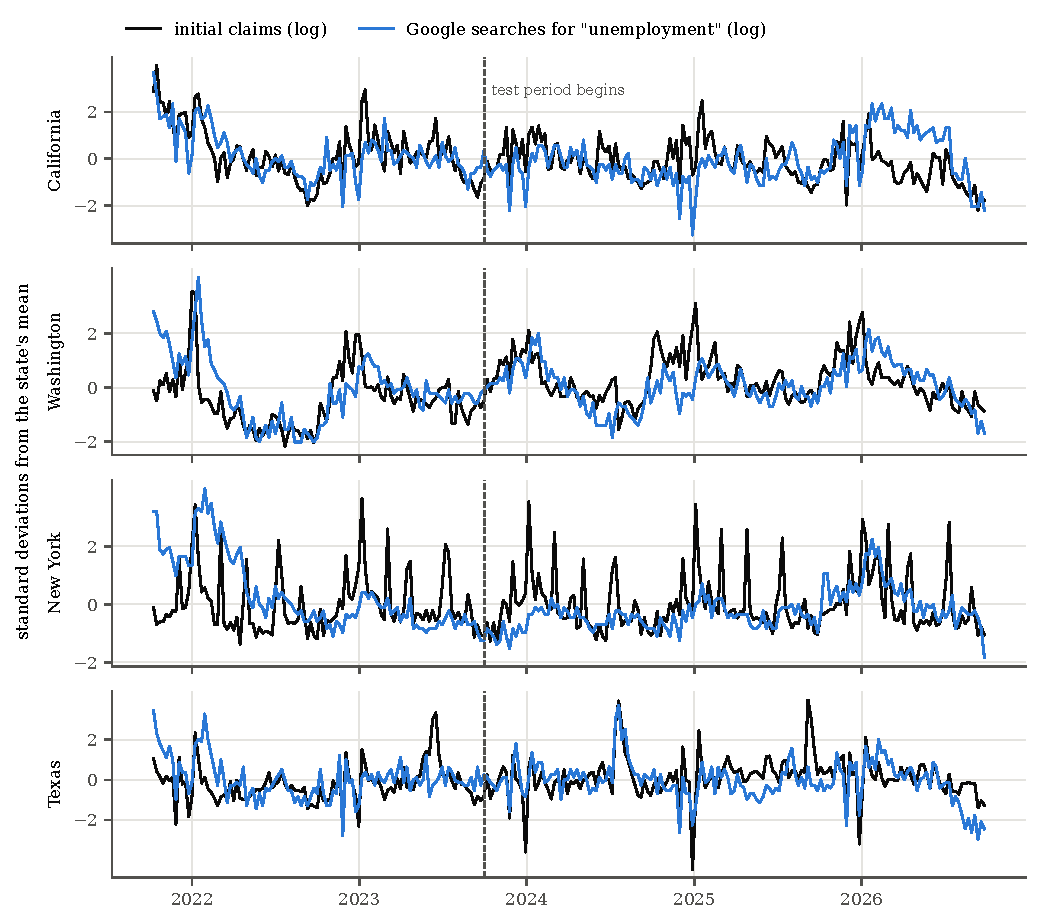
\includegraphics[width=0.9\textwidth]{../out/figures/fig1_series.pdf}
  \caption{Weekly initial claims and Google searches for ``unemployment'' in each state,
  both in logs and standardized. The two move together most visibly at the turn of each
  year, which is why a fair test has to give the baseline the calendar. Models are fit on
  weeks before the dashed line and scored on weeks after it.}
  \label{fig:series}
\end{figure*}

Figure~\ref{fig:series} shows claims and searches over the study period.

\textbf{Reddit.} We downloaded all $43{,}870$ posts in r/Unemployment over the window from
the Arctic Shift archive~\cite{arcticshift}. The subreddit asks posters to tag their state
in the flair or title, for example ``[California] Question''. We assign a post to a state by
that tag, or, when there is none, if its title or body names exactly one of our states or its
unemployment agency (EDD, ESD, NYSDOL, TWC). We hand-checked 40 randomly chosen posts from
the first months of the download and found no misassignments. Posts tagged ``[All States]'' count toward no state. The result is
uneven: $19.9$ posts per week for California, $16.8$ for New York, $7.4$ for Texas, and
$2.5$ for Washington. For the tech hypothesis we use the daily post count of
r/cscareerquestions, about $920$ posts per week.

\section{The Question and How It Changed}

Our proposal asked: \emph{do job-loss searches and Reddit discussions improve estimates of
weekly state-level initial claims beyond what past claims already tell us}, and does
tech-related Reddit discussion help more in California and Washington? The main question
did not change. Four things around it did.

\textbf{r/layoffs had to be dropped.} The proposal named r/layoffs as a tech signal. The
subreddit had $2$ posts in 2021, $18$ in 2022, and $528$ in 2023, against $6{,}126$ in
2024. A regressor that is zero for the first two years cannot be trained. The tech
hypothesis is tested with r/cscareerquestions alone.

\textbf{``Explicit state mentions'' became the subreddit's own tags.} Searching post text
for state names was the plan. Once we saw that most posts carry a state flair, the flair was
the more reliable signal, and text matching became the fallback.

\textbf{The baseline needed the calendar.} Our first baseline used last week's change and
the same week's change a year earlier. Its largest errors in the training period fell on
holidays that move against a 52-week lag: Thanksgiving, New Year, and Easter, which drives
large spring spikes in New York. We added holiday terms, choosing them using the training
period only.

\textbf{A second question emerged: where does the gain come from?} Once Trends helped on
average, we wanted to know whether it helped every week or a few. The answer, a few, turned
out to be the most informative finding.

\section{Method}

\textbf{Target and timing.} Each model predicts the week-over-week change in log claims,
$\Delta y_t = \log c_t - \log c_{t-1}$, from information available on the Sunday after week
$t$ ends: claims through week $t-1$ and online activity through week $t$. A nowcast of
$\Delta y_t$ gives a nowcast of $c_t$, five days before the official number. Errors are in
log points, which are roughly percent.

\textbf{Baseline.} $\Delta y_t$ regressed on $\Delta y_{t-1}$, the year-ago change
$\Delta y_{t-52}$, and, for each of Thanksgiving, Christmas, New Year's Day, and Easter, an
indicator of whether the holiday falls in week $t$ but not week $t-52$ (or the reverse), for
the holiday week and the week after. We compared this with simpler alternatives in an
expanding-window evaluation inside the training period only, and fixed it before looking at
the test period.

\textbf{Augmented models.} Each adds this week's change in one online signal, in logs, to
the baseline. \emph{Trends} adds all three search terms jointly. \emph{Reddit} adds the
state's r/Unemployment posts. \emph{Tech} adds r/cscareerquestions posts. All were specified
before the test period was evaluated.

\textbf{Evaluation.} Training starts with the week ending October 16, 2021. For each test
week from October 7, 2023 to September 26, 2026 (156 per state), every model is re-estimated
by least squares on all earlier weeks ($103$ at the first test week) and predicts that week.
We report the reduction in mean squared error (MSE) relative to the baseline. Because each
augmented model contains the baseline, we test it with the Clark--West
statistic~\cite{clark2007approximately}. The usual Diebold--Mariano
test~\cite{diebold1995comparing} is biased against the larger model in this nested setting.
We use one-sided $p$-values with Newey--West variance. Pooled results average the four
states' loss differentials within each week before testing.

\section{Results}

\begin{table}[t]
  \caption{Out-of-sample reduction in squared nowcast error relative to the baseline, 156
  weeks per state. Clark--West $p$-values in parentheses. Baseline RMSE is in log points.}
  \label{tab:main}
  \small
  \begin{tabular}{lrrrr}
    \toprule
              & Baseline & + Trends & + Reddit & + Tech \\
              & RMSE     & (\%)     & (\%)     & (\%)   \\
    \midrule
    California & 8.8  & 23.2 (.000) & $-1.6$ (.87) & $-1.8$ (.93) \\
    Washington & 9.9  & $-0.7$ (.057) & 1.5 (.15) & $-0.5$ (.96) \\
    New York   & 20.8 & 6.7 (.001) & 2.0 (.052) & 0.6 (.24) \\
    Texas      & 16.0 & 22.1 (.001) & 1.3 (.064) & $-1.4$ (.98) \\
    \midrule
    Pooled     & 14.7 & 11.9 (.000) & 1.4 (.006) & $-0.3$ (.39) \\
    \bottomrule
  \end{tabular}
\end{table}

\begin{figure}[t]
  \centering
  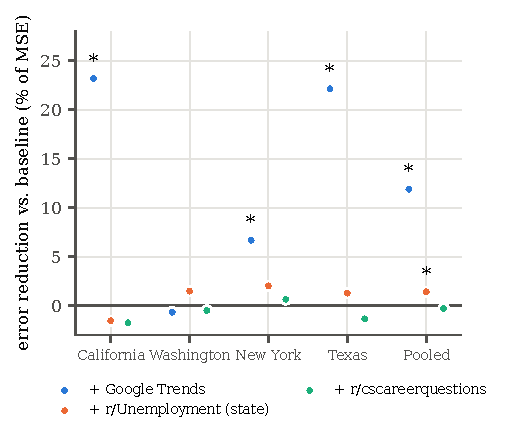
\includegraphics[width=\columnwidth]{../out/figures/fig2_accuracy.pdf}
  \caption{Reduction in out-of-sample squared error from adding each online signal to the
  baseline. An asterisk marks Clark--West $p<0.05$.}
  \label{fig:accuracy}
\end{figure}

\subsection{Google searches help, but not everywhere}

Table~\ref{tab:main} and Figure~\ref{fig:accuracy} give the main result. Adding Google
Trends reduces squared nowcast error by $11.9\%$ pooled across the four states
($p<0.001$), and the pooled root-mean-square error falls from $14.7$ to $13.8$ log points.
The gain is large in California ($23.2\%$) and Texas ($22.1\%$), smaller in New York
($6.7\%$), and absent in Washington ($-0.7\%$).

The term matters more than we expected. ``File for unemployment'', which states the
intention most directly and which our proposal led with, adds nothing on its own when
pooled ($-0.6\%$, $p=0.33$). The broad term ``unemployment'' carries the gain on its own
($13.3\%$), and ``unemployment benefits'' adds $5.1\%$. A plausible reason is volume: the
specific phrase is rarer, so Trends' sampled index is noisier, and in Washington it is
suppressed to zero in a third of weeks. Even the broad term adds only $0.3\%$ in Washington,
the smallest state, which suggests that sampling noise limits Trends in smaller states.

\begin{figure*}[t]
  \centering
  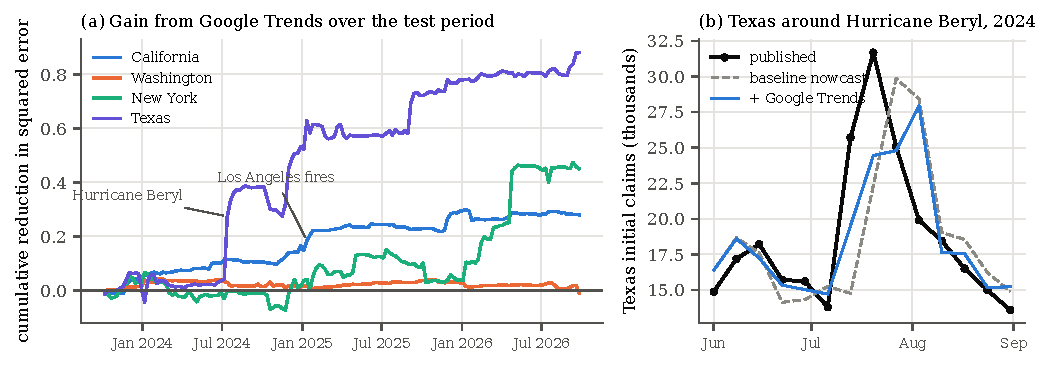
\includegraphics[width=0.9\textwidth]{../out/figures/fig3_where.pdf}
  \caption{(a) Cumulative reduction in squared nowcast error from adding Google Trends, over
  the test period. Flat stretches are weeks where the two models agree; the jumps are a few
  weeks with large shocks. (b) Texas around Hurricane Beryl (landfall July 8, 2024): weekly
  claims, and the nowcasts each model made before the official number was released.}
  \label{fig:where}
\end{figure*}

\subsection{The gain comes from a few weeks}

Pooled, the Trends model is closer to the truth in only $53.4\%$ of weeks, barely more than
a coin flip. Figure~\ref{fig:where}a shows why the average gain is still large: cumulative
gain is flat most of the time and rises in steps. The ten best weeks account for $87.2\%$ of
California's total gain and all of Texas's.

The largest single step is Hurricane Beryl. In the week ending July 13, 2024, Texas claims
rose by $62.3$ log points as power outages closed businesses around Houston. The baseline,
which knows only the calendar and the previous week, missed by $55.5$ log points. The Trends
model missed by $27.6$, halving the error, because searches for unemployment rose the same
week (Figure~\ref{fig:where}b). That one week is $26.3\%$ of Texas's gain over three years.
The Los Angeles wildfires in January 2025 show the same pattern on a smaller scale: claims
rose $26.7$ log points, and the Trends model's error was $19.9$ log points instead of
$27.6$.

Other steps are holidays. Two of California's five best weeks are Thanksgiving weeks and a
third is Christmas week: filing drops because offices close, and searches drop with it. Our holiday terms
correct for the holiday's date but not for how strong its effect is in a given year, and
searches capture some of that. Excluding every holiday week and the week after it, the
Trends gain falls from $11.9\%$ to $7.9\%$, and it remains significant ($p<0.001$). Roughly
a third of the average gain is therefore holiday timing, which a better calendar model could
in principle capture, and the rest is information the calendar does not have.

\subsection{Reddit adds little}

Posts in r/Unemployment tagged with a state reduce error by $1.4\%$ pooled. The gain is
small but statistically distinguishable from zero ($p=0.006$), and no single state is
significant at $0.05$. Adding Reddit to Trends raises the pooled gain from $11.9\%$ to
$12.7\%$. The obstacle is volume. Even California averages $19.9$ tagged posts per week,
too few for week-to-week changes to say much about tens of thousands of filings, and many
posts concern ongoing claims rather than new ones.

\subsection{The tech hypothesis is not supported}

We expected r/cscareerquestions to help most in California and Washington, where tech
employment is concentrated. It helps in no state: $-1.8\%$ in California, $-0.5\%$ in
Washington, $0.6\%$ in New York, and $-1.4\%$ in Texas. Tech workers are a small share of
claimants even in those states, and laid-off tech workers often receive severance and file
weeks later, if at all. A subreddit mostly about careers and job searching is also only
loosely tied to job loss.

\subsection{Robustness}
\label{sec:robust}

\begin{table}[t]
  \caption{Pooled reduction in squared error from adding Google Trends, under variations of
  the design. Clark--West $p$-values in parentheses.}
  \label{tab:robust}
  \small
  \begin{tabular}{lr}
    \toprule
    Variation & Reduction (\%) \\
    \midrule
    Main specification                          & 11.9 (.000) \\
    Weak baseline (no seasonal or holiday terms) & 17.5 (.000) \\
    Last week's claims not yet published         & 13.0 (.000) \\
    Rolling 104-week estimation window           & 8.7 (.000) \\
    Excluding holiday weeks and the week after   & 7.9 (.000) \\
    Test year Oct 2023 -- Sep 2024               & 14.7 (.012) \\
    Test year Oct 2024 -- Sep 2025               & 8.5 (.006) \\
    Test year Oct 2025 -- Sep 2026               & 16.0 (.000) \\
    \bottomrule
  \end{tabular}
\end{table}

Table~\ref{tab:robust} reruns the comparison under alternative designs. The gain is positive
and significant in every variation. It is larger against a weak baseline without seasonal
or holiday terms ($17.5\%$). This is the Google Flu Trends lesson in miniature: against a
baseline that does not know the calendar, part of what searches appear to add is the
calendar. When the previous week's claims are not yet published, which happened on $10.6\%$
of Sundays, the gain is $13.0\%$, about the same as when they are. A rolling two-year
window gives a smaller gain ($8.7\%$) than the expanding window. The gain is present in each
of the three test years.

Searches are also not simply correlated with claims. Over the whole window, the correlation
between log claims and log searches for ``unemployment'' ranges from $0.28$ in New York to
$0.58$ in Washington, and Washington, where the correlation is highest, is where searches
add nothing out of sample. Correlation in levels does not indicate whether a signal will
improve a forecast.

\section{Limitations}

\textbf{Trends is not a real-time source.} We downloaded the whole five-year series in
November 2026. A forecaster in 2024 would have seen a different sample, scaled to a
different peak, and Trends data cannot be re-downloaded identically. Our results therefore
assume that the search index available in real time behaves like the one we downloaded. The
re-scaling itself does not matter, because the models use weekly changes in logs, but the
sampling does. We tried to measure sampling noise by downloading again; within a day the
results were identical, apparently cached, so we could not.

\textbf{Few events drive the result.} With most of the gain in a handful of weeks, a
different three years could give a larger or smaller number. The finding generalizes as
``searches help most when something unusual happens'', not as a fixed percentage.

\textbf{Four states.} We chose the states for the tech hypothesis, not as a sample of the
country. Washington's result suggests that Trends works less well in smaller states, but
one state is not enough to establish that.

\textbf{State tags are not residence.} A Reddit post tagged ``[Texas]'' is about Texas
unemployment, not necessarily by a Texan. This adds noise to an already weak signal.

\section{What We Did}

Most of the work was getting data we could trust. Trends has no open API, and automated
requests are blocked. We exported the twelve series through a browser and checked each
transcribed series against checksums computed in the page. Reddit came from a community
archive whose API timed out intermittently, so the download scripts had to resume after
interruptions. For the high-volume r/cscareerquestions we switched to the archive's daily
counts, after checking that they matched a week of individually downloaded posts exactly.
We downloaded every Sunday's version of each claims series to check revisions and
publication lags, rather than assuming them.

Things that did not work: r/layoffs, which barely existed before 2024; the proposal's lead
search term; the tech hypothesis; a seasonal term averaged over several pre-pandemic years,
which did worse in the training period than last year's alone because seasonal patterns
changed after 2020; and measuring Trends sampling noise.

\section{Conclusion}

Google searches contain a usable signal about state unemployment claims, five days before
the official number. Added to a baseline that already knows past claims and the calendar,
they reduce squared nowcast error by about $12\%$ across four states, and they remain
useful when official data are a week staler than usual. The gain is uneven. It is large in
California and Texas and absent in Washington, and it comes from a few weeks: holidays, a
hurricane, and a wildfire. In ordinary weeks, searches add almost nothing to what last week
and last year already predict. Reddit, at the volumes available for a single state, adds
little, and tech-career discussion adds nothing for the states where we expected it to
matter.

For anyone using these signals in practice, the practical value of search data is in the
weeks when official data are most out of date and the situation changes faster than any
calendar model can anticipate, which are the weeks a nowcast matters most.

\bibliographystyle{ACM-Reference-Format}
\bibliography{refs}

\end{document}
